\documentclass[a4paper, 12pt, oneside]{book}
\usepackage{graphicx}
\usepackage[french]{babel}
\usepackage[utf8]{inputenc}
\usepackage[T1]{fontenc}
\frenchbsetup{StandardLists=true}
\usepackage{enumitem}
\usepackage{multirow}
\usepackage{listings}
\usepackage{float}
\usepackage{hyperref}
\usepackage{amsmath}
\usepackage{amssymb}
\usepackage{url}
\usepackage[french]{algorithm}
\usepackage{style/myalgorithm}
\usepackage{amsmath,amsfonts,amssymb}
\newcommand{\fBm}{\emph{fBm}~}
\newcommand{\etal}{\emph{et al.}~}
\newcommand{\glAd}{\emph{GL4D}~}
\newcommand{\apiopengl}{API OpenGL\textsuperscript{\textregistered}~}
\newcommand{\opengl}{OpenGL\textsuperscript{\textregistered}~}
\newcommand{\opengles}{OpenGL\textsuperscript{\textregistered}ES~}
\newcommand{\clang}{langage \texttt{C}}
\newcommand{\codesource}{\textsc{Code source}~}
\floatstyle{ruled}
\newfloat{programslist}{htbp}{locs}
\newcommand{\listofprograms}{\listof{programslist}{Liste des codes source}}
\newcounter{program}[subsection]
\renewcommand{\theprogram}{\arabic{chapter}.\arabic{program}}

\newenvironment{program}[1]{
  \if\relax\detokenize{#1}\relax
  \gdef\mycaption{\relax}
  \else
  \gdef\mycaption{#1}
  \fi
  \refstepcounter{program}
  \addcontentsline{locs}{section}{#1}
  \footnotesize
}{
  \begin{description}
    \item[\codesource \theprogram]--~\mycaption
  \end{description}
}

\begin{document}
\begin{titlepage}
  \begin{center}
    \begin{tabular*}{\textwidth}{l@{\extracolsep{\fill}}r}
      
\includegraphics[height=1.5cm]{images/m1info.png}&
      
\includegraphics[height=1.5cm]{images/oaccueil.png}
    \end{tabular*}
    \small 
    \rule{\textwidth}{.5pt}~\\
    \large 
    \textsc{Université Paris 8 - Vincennes à Saint-Denis}\vspace{0.5cm}\\
    \textbf{M1 MIASHS : Big Data et fouille de données}\vspace{3.0cm}\\
    \Large
    \textbf{Projet: Random Forest}\vspace{1.5cm}\\
    \large
    \textbf{PANCHALINGAMOORTHY \textsc{Gajenthran}, LABAT Kaxandra}\vspace{1.5cm}\\
  \end{center}\vspace{1.5cm}~\\
  \begin{tabular}{ll}
    \hspace{-0.45cm}Organisme d'accueil~:~&~Université Paris 8\\
    \hspace{-0.45cm}Cours ~:~&~Décision et parcours espace de données\\
  \end{tabular}
\end{titlepage}
\frontmatter

\mainmatter

%% Introduction
\chapter[Exercices]{Introduction}



\section{Exercice 1}
\textit{Quelles les prétraitements obligatoires avant d’appliquer l’algorithme Random Forest de Python (Package SkLearn)?}
\newline \newline
Avant de commencer à appliquer l'algorithme Random Forest, il faut tout d'abord commencer par importer le package \texttt{sklearn} et réaliser la commande suivante afin d'importer le module Random Forest: \texttt{from sklearn.ensemble import RandomForestClassifier}.
De plus, pour appliquer notre algorithme Random Forest, il faudra éventuellement un ensemble de données pour pouvoir l'exploiter. C'est pourquoi nous allons nous charger d'importer le contenu du fichier \textit{CarteBanquaire.csv}. La méthode \texttt{read\_csv} du module \texttt{pandas}, fera largement l'affaire pour lire ce fichier.
\newline
Dans le cas où nous souhaiterons vérifier notre classifieur, nous séparerons notre base de données en 2 parties: une partie pour l'apprentissage et l'autre pour la phase d'entraînement, à l'aide de \texttt{train\_test\_split} provenant de \texttt{sklearn.model\_selection}. À noter qu'il est important de bien distinguer la colonne \textit{Class} lors de la séparation des données.
\newline \newline
Liste des modules utilisés:
\begin{verbatim}
import pandas as pd
from sklearn.model_selection import train_test_split
from sklearn.ensemble import RandomForestClassifier
\end{verbatim}



\section{Exercice 2}
\textit{Trouver le meilleur paramétrage afin d’avoir le taux d’erreur minimum sur le classifieur}
\newline \newline
Un des prétraitements intéressants avant l'utilisation finale du Random Forest, semble être le \texttt{GridSearchCV}. Cet élément là, va nous permettre de pouvoir utiliser les paramètres les plus efficaces pour notre modèle afin d'obtenir les meilleurs résultats. Tout d'abord, avant d'utiliser le \texttt{GridSearchCV}, le choix des paramètres pour les tests sont à fixer. Le nombre de paramètres à tester influencera sur le temps d'exécution. Les paramètres qui semblent les plus judicieux pour le \texttt{GridSearchCV} paraissent être \texttt{n\_estimator}, \texttt{max\_depth}, \texttt{min\_samples\_split} et \texttt{min\_samples\_leaf}. Nous pourrions en rajouter d'autres, mais cela prendrait trop de temps. 
\begin{itemize}
\item \texttt{n\_estimators} représente le nombre d'arbres de décision dans le modèle. Il a donc un impact important sur la qualité de l'apprentissage des données; en effet, plus la forêt a d'arbres, plus la qualité de l'apprentissage sera importante. Mais cela a aussi un effet sur le temps d'exécution de notre programme qui est un élément à prendre en compte: il est donc essentiel de trouver la bonne valeur pour trouver le juste milieu entre le coût et la performance. 
\item \texttt{max\_depth} représente la profondeur de chaque arbre dans la forêt. Plus l'arbre est profond, plus on aura d'informations à propos des données.
\item \texttt{min\_samples\_split} représente le nombre minimal d'échantillons nécessaire pour diviser un noeud interne. Plus cette valeur augmente, plus chaque arbre dans la forêt considérera plus d'échantillons à chaque noeud. Nous avons le choix entre mettre un flottant ou un entier pour cette valeur: si il s'agit d'un entier, cela correspondra au nombre minimum d'échantillons; si il s'agit d'un flottant, cela correspondra au pourcentage d'échantillons.
\item \texttt{min\_samples\_leaf} représente le nombre minimal d'échantillons nécessaire pour être au niveau d'un noeud feuille.
\end{itemize}
\begin{verbatim}
param_grid = {
    "n_estimators": [10, 50, 100],
    "max_depth": [5, 8, 15],
    "min_samples_split": [2, 5, 10, 30],
    "min_samples_leaf": [1, 2, 5, 10]
}
\end{verbatim}
Pour traduire ce dictionnaire \texttt{param\_grid}, les clés correspondent aux paramètres de Random Forest, et les valeurs sont des tableaux dans lesquels chaque valeur est une valeur d'un paramètre. Par exemple, nous allons tester, RandomForestClassifier avec le paramètre \texttt{n\_estimators} qui prendra les valeurs 10, 50, 100. 
Outre la spécification de l'estimator, en l'occurence ici notre Random Forest, et les paramètres dont nous voulons tester, il existe d'autres paramètres du \texttt{GridSearchCV} que nous pouvons régler.
\newline
Vous trouverez un aperçu de l'ensemble des résultats du \texttt{GridSearchCV} sur le fichier \textit{gridsearchcv.txt}.
\begin{verbatim}
def tuning_rfc_param(param_grid, rfc, X, y):
    CV_rfc = GridSearchCV(
        estimator=rfc, 
        param_grid=param_grid,
        verbose=1,
        n_jobs=-1,
        cv=2)

    CV_rfc.fit(X, y)
\end{verbatim}

Liste des modules utilisés: 
\begin{verbatim}
from sklearn.model_selection import GridSearchCV
\end{verbatim}



\section{Exercice 3}
\textit{Quel est le taux d'erreur de votre modèle random forest ?}
\newline \newline
Avec le \texttt{GridSearchCV}, nous remarquons que le taux d'erreur de notre meilleur classifieur est de 0.999567 avec les paramètres suivants: \texttt{\{'max\_depth': 15, 'min\_samples\_leaf': 1, 'min\_samples\_split': 2, 'n\_estimators': 50\}}.



\section{Exercice 4}
\textit{Quel est le meilleur classifieur (ou estimator) de votre random forest ?}
\newline \newline
Pour récupérer les estimators de notre Random Forest, il faut d'abord connaître la valeur que nous avons attribuée à \texttt{n\_estimator}; en effet, comme nous l'avons vu précédemment \texttt{n\_estimator} nous indique le nombre d'arbres utilisés pour le modèle, et plus précisément il nous indique le nombre de \texttt{DecisionTreeClassifier} que l'on va utiliser. On peut accéder à chaque arbre avec l'attribut \texttt{estimators} de \texttt{RandomForestClassifier}, une fois la classification réalisée; cet attribut nous renvoie une liste de \texttt{DecisionTreeClassifier} dont le nombre d'éléments est équivalent à \texttt{n\_estimator}. Pour savoir lequel des estimators est le plus performant, nous allons tester chacun des estimators avec notre test de données et utiliser une méthode permettant de calculer les taux d'erreur comme \texttt{MSE} (Mean Squared Error), \texttt{MAE} (Mean Absolute Error), \texttt{RMSE} (Root Mean Squared Error)...
\begin{verbatim}
def calculate_estimators_errors(rfc, X, y, debug=True):
    estimator_errors = []
    for tree in rfc.estimators_:
        pred = tree.predict(X)
        estimator_errors.append(mean_squared_error(y, pred))

    return estimator_errors.index(max(estimator_errors))
\end{verbatim}
On obtient ainsi l'estimator le plus performant à l'indice 35 avec un taux d'erreur de 0.0006056722523107713.
\newline \newline
Liste des modules utilisés:
\begin{verbatim}
from sklearn.metrics import mean_squared_error
\end{verbatim}



\section{Exercice 5}
\textit{Affichez le taux d’erreur de tous les estimator de votre modèle Random Forest}
\newline \newline
Voici la liste du taux d'erreur des estimators du Random Forest:
\begin{verbatim}
[0.0007548958507061788, 0.0007812294268936036, 0.0009655644602055774, 
 0.000974342318934719, 0.0007724515681644619, 0.0007548958507061788, 
 0.0007197844157896123, 0.0008338965792684533, 0.0008690080141850197, 
 0.0007636737094353204, 0.0008075630030810285, 0.0007636737094353204,
 0.0007987851443518868, 0.0007110065570604707, 0.0007636737094353204, 
 0.0008602301554558781, 0.0009831201776638607, 0.0007548958507061788, 
 0.0006232279697690545, 0.0007724515681644619, 0.000702228698331329, 
 0.0008338965792684533, 0.0007110065570604707, 0.0009480087427472942, 
 0.0008777858729141613, 0.0009128973078307278, 0.00081634086181017, 
 0.0009480087427472942, 0.0006320058284981962, 0.0006934508396021874, 
 0.00081634086181017, 0.0009918980363930023, 0.0008777858729141613, 
 0.0008075630030810285, 0.0008690080141850197, 0.0006056722523107713,
 0.0007636737094353204, 0.0009128973078307278, 0.0007285622745187538, 
 0.0008514522967267364, 0.00081634086181017, 0.0007461179919770371, 
 0.0007373401332478955, 0.0008338965792684533, 0.0007548958507061788, 
 0.0007724515681644619, 0.00081634086181017, 0.00081634086181017, 
 0.0007461179919770371, 0.0008690080141850197]
\end{verbatim}



\section{Exercice 6}
\textit{Prenez deux estimators de votre modèle Random Forest, l'estimator le plus performant et l'estimator le moins performant. Quel est le taux d'erreur des deux estimatiors}
\newline \newline
Il s'agit du même procédé que pour chercher l'estimator le plus performant
\begin{verbatim}
def calculate_estimators_errors(rfc, X, y, debug=True):
    estimator_errors = []
    for tree in rfc.estimators_:
        pred = tree.predict(X)
        estimator_errors.append(mean_squared_error(y, pred))

    return estimator_errors.index(min(estimator_errors)),
           estimator_errors.index(max(estimator_errors))
\end{verbatim}
On obtient donc un taux d'erreur de 0.0006056722523107713 pour l'estimator le plus performant contre 0.0009918980363930023 pour l'estimator le moins performant



\section{Exercice 7}
\textit{Quelle est la différence entre la moyenne des taux d'erreur des deux estimators et le taux d'erreur de votre meilleur modèle random Forest ?}
\newline \newline
Soit \texttt{M\_EE}, la moyenne du taux d'erreur des deux estimators, \texttt{ER}, le taux d'erreur du Random Forest et \texttt{DIFF\_E}, la différence entre \texttt{ER} et \texttt{M\_EE}
\newline
\texttt{M\_EE = \begin{equation} \frac{0.0006056722523107713 + 0.0009918980363930023}{2} \end{equation} = 0.0007987851443518868}
\newline
\texttt{ER = 0.00036867006662394777}
\newline
\texttt{DIFF\_E = 0.0007987851443518868 - 0.00036867006662394777 = 0.000430115077727939}
\newline \newline
On remarque grâce à cette valeur, on obtient souvent la même valeur (en répétant cette action plusieurs, nous pouvons plus ou moins arriver à cette conclusion, avec une valeur avoisinant les 0.0004). Ainsi la différence entre la moyenne des taux d'errreur des deux estimators et le taux d'erreur de notre modèle peut se percevoir sur le fait que le taux d'erreur du modèle correspond plus à une moyenne de l'ensemble des arbres plutôt qu'un de ces deux estimators.

 

\section{Exercice 8}
\textit{Affichez les deux arbres correspondants au deux estimators}
\newline \newline
Pour pouvoir visualiser un arbre, il faudra utiliser la méthode \texttt{export\_graphviz} de \texttt{sklearn.tree}. Cette dernière peut prendre des arguments tels que l'estimator qu'on souhaite visualiser, le fichier de sortie pour stocker l'arbre, les fonctionnalités (dans notre cas V1, V2, V3... V20, Time et Amount), et la classe qu'on obtient.
\begin{verbatim}
def vizualize_estimators(estimators, out_files, feature_names, class_names):
    for i in range(0, len(estimators)):
        export_graphviz(
            estimators[i],
            out_file=out_files[i],
            feature_names=feature_names,
            class_names=class_names
        )
\end{verbatim}
Cependant, il faut prendre en compte que cette fonction nous donne un fichier \textit{.dot} que l'on peut convertir en \textit{.png} pour le visualiser.
\newline \newline
Liste des modules utilisés:
\begin{verbatim}
from sklearn.tree import export_graphviz
\end{verbatim}


  \begin{figure}[H]
    \centering
    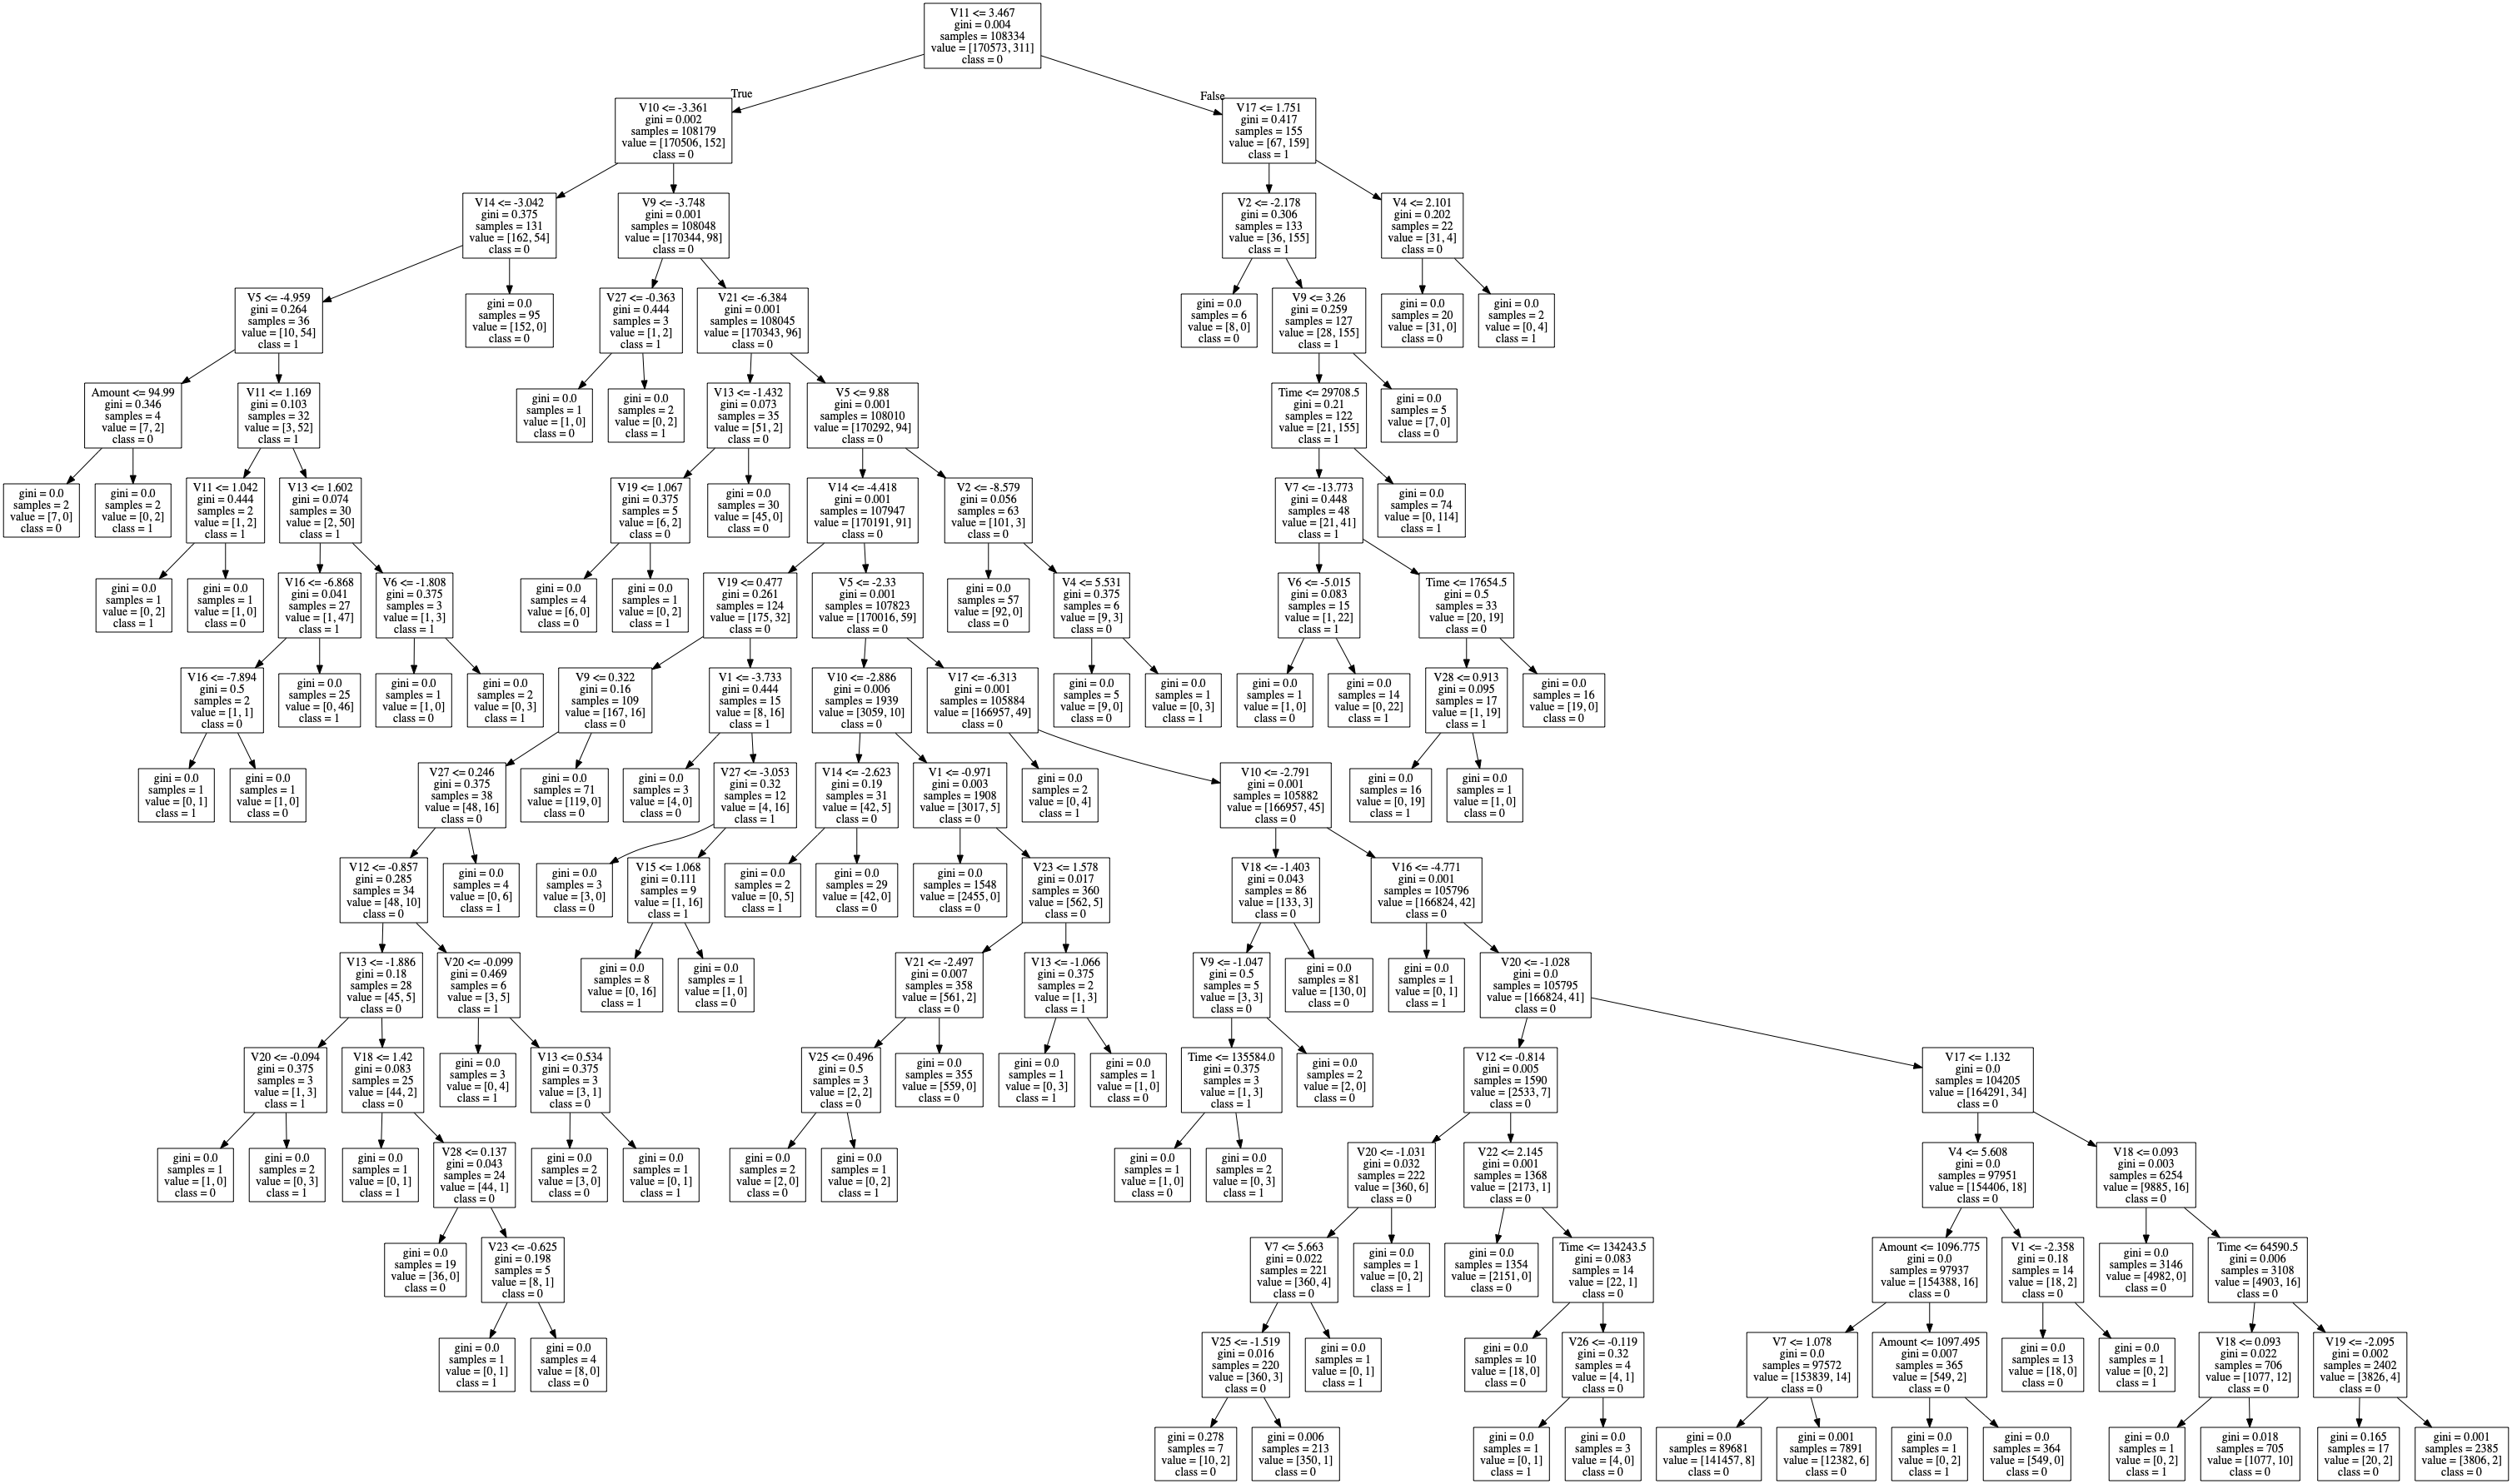
\includegraphics[width=0.8\textwidth]{images/best_tree}
    \caption{Arbre pour l'estimator pour le plus performant}
    \label{fig:intro-home}
  \end{figure}


  \begin{figure}[H]
    \centering
    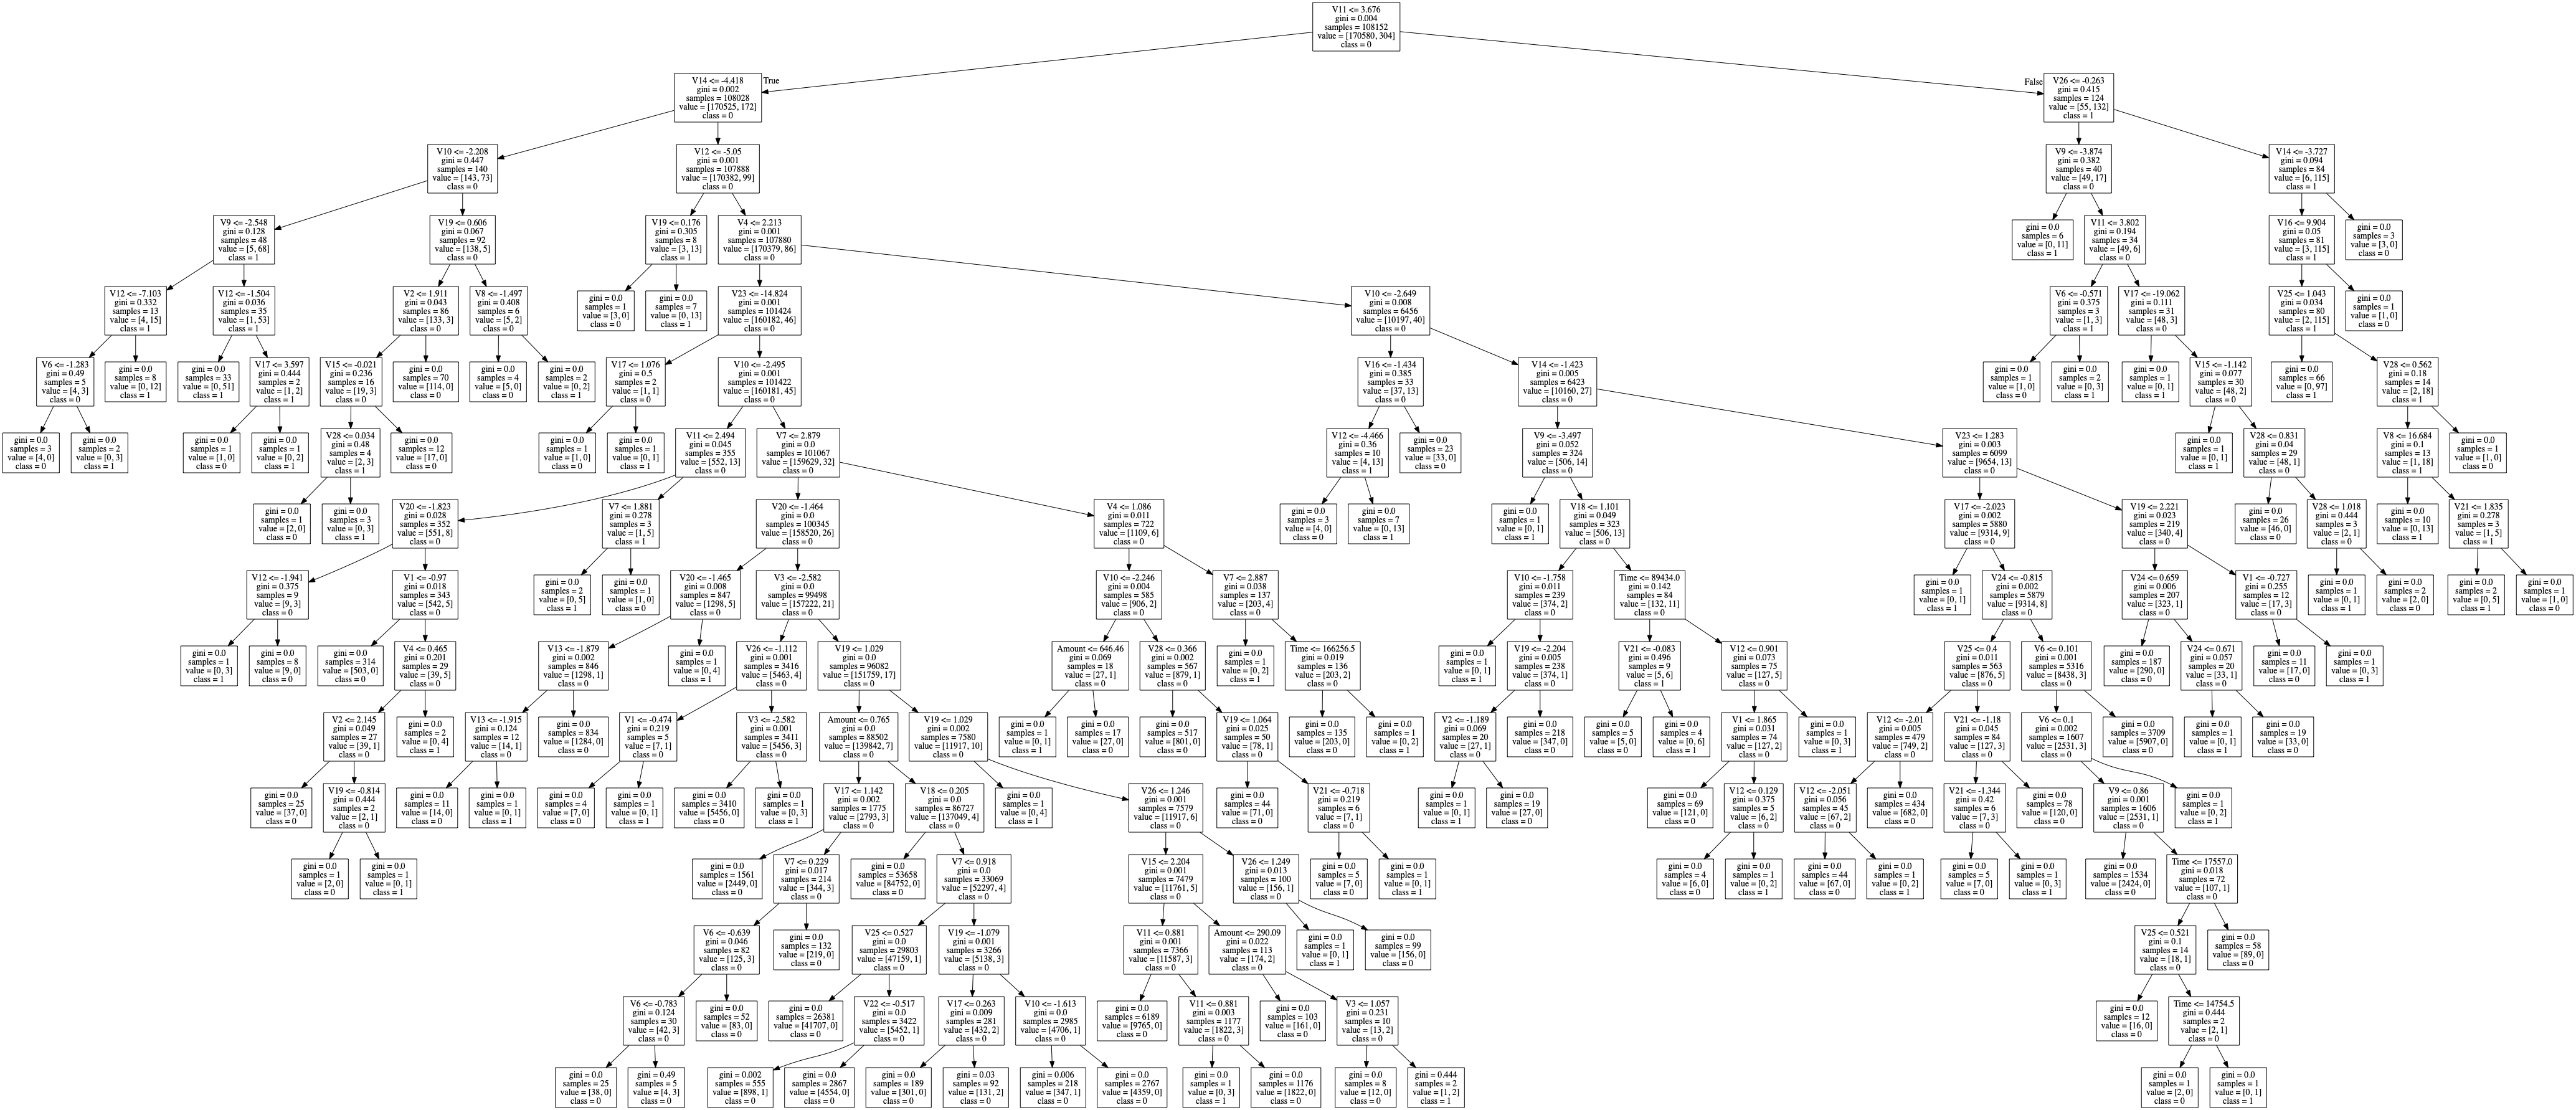
\includegraphics[width=0.8\textwidth]{images/worst_tree}
    \caption{Arbre pour l'estimator pour le moins performant}
    \label{fig:intro-home}
  \end{figure}



\section{Exercice 9}
\textit{Ecrire la liste des règles de décision extraites des deux estimator sous forme de Si A , B => C (x \%) ?}
\newline \newline
Vous pouvez trouver les règles de decision des deux arbres dans les fichiers suivants: \textit{worst\_tree\_rules.txt} et \textit{best\_tree\_rules.txt}.

\section{Exercice 10}
\textit{Quelles les règles dont un besoin le mauvais estimator pour qu'il s'approche des performances du bon estimator ?}
\newline \newline
Les règles permettant d'améliorer un mauvais estimator sont principalement le choix des premiers attributs pour la racine de l'arbre; cela va aider à ce que la structure de l'arbre soit la plus optimale posible. De plus le pruning de certaines branches peut permettent d'obtenir un estimator plus efficace.

\bibliographystyle{alpha}
\bibliography{memoire}
\end{document}
